\documentclass{rapportECL}
\usepackage{lipsum}
\usepackage{hyperref}
\documentclass{book}
\usepackage[utf8]{inputenc}
\usepackage[french]{babel}
\usepackage{tikz}
\title{Rapport} 

\begin{document}

%----------- Informations du rapport ---------

\titre{Rapport Conception Logiciel 2}
\UE{4ème Semestre}
\sujet{Licence Informatique} 

\enseignant{Yann \textsc{Mathet}} 

\eleves{  \textsc{Janest}  Jérôme \\
             \textsc{Lejemtel} Antoine\\
             \textsc{Gurita} Louis    \\
	    }

%----------- Initialisation -------------------
        
\fairemarges
\fairepagedegarde
\tabledematieres 

%------------ Corps du rapport ----------------

\section{Introduction}
Par groupe de 4, il nous a été demandé de réaliser une des applications proposées, sur différents thèmes : jeux vidéos, sténographie, etc.
\newline
\newline
Pour notre groupe le choix de notre sujet était évident, le Ricochet Robots était complémentaire de notre projet au 3ème semestre en "Introduction à la POO" qui était de développer un morpion et le jeu de Nim avec leurs IA. La suite logique était donc de continuer sur le développement et l'apprentissage d'un autre genre d'IA, celle du Ricochet Robots dont l'énoncé est la suivante:
\newline
\newline
\emph{
"Le principe du jeu de société Ricochet Robots est de trouver en moins d'une minute la séquence de mouvement qui permettra à un robot donné (parmi quatre) d'atteindre un objectif désigné sur une case du plateau de jeu. Cependant, les robots ne peuvent que se déplacer en ligne droite jusqu'à rencontrer un obstacle. Le but de ce projet est de développer un programme permettant de trouver une solution optimale pour toute situation du jeu. Dans un premier temps, il s'agira de développer le moteur du jeu puis d'implanter un algorithme de résolution, appelé A*. Cependant, le problème est trop complexe pour être résolu dans de bonnes conditions. Dans un second temps, il s'agira alors de proposer des méthodes d'optimisation de l'algorithme, par exemple en utilisant des tables de transposition. Enfin, s'il reste du temps, il pourra être intéressant de réaliser une interface graphique permettant à un utilisateur de sélectionner un objectif."}
\newline
\newline
Nous avons adapté notre version du jeu physique au numérique, dont nous allons détailler les différences plus tard dans le rapport.
\newline
\newline
Notre projet a été divisé en 3 parties : 

\begin{itemize}
\item Le développement d'objets permettant de stocker dans une grille les différents paramètres et méthodes nécessaires, au bon fonctionement du programme.
\item Le développement de l'affichage en utilisant les librairies "JFrame" et "Canvas".
\item Implémentation de l'intelligence artificielle, en passant par plusieurs niveaux.
\end{itemize}

\newpage
\newpage

\section{Ricochet Robots}
Ricochet Robots (Rasende Roboter pour la première édition en allemand) est un jeu de société créé par Alex Randolph et illustré par Franz Vohwinkel, édité en 1999 par Hans im Glück / Tilsit.
\newline
Le jeu est composé d'un plateau, de tuiles représentant chacune une des cases du plateau, et de pions appelés « robots ». La partie est décomposée en tours de jeu, un tour consistant à déplacer les robots sur un plateau afin d'en amener un sur l'une des cases du plateau. Les robots se déplacent en ligne droite et avancent toujours jusqu'au premier mur qu'ils rencontrent.
\newline
L'objectif du jeu consiste à récupérer des pion d'objectif en amenant un des robots sur une case particulière du plateau.
\newline
Le but est alors d'amener le robot de la couleur du pion d'objectif sur la case de celui-ci. 
\newline
\newline
Les joueurs jouent simultanément, chacun réfléchissant sur le moyen d'amener le robot en utilisant les règles de déplacement. Lorsque l'un d'entre eux pense avoir trouvé une solution, il annonce en combien de mouvements il compte réaliser l'objectif puis il lance un timeur. Les autres joueurs ont jusqu'à la fin du sablier pour proposer de meilleures solutions, utilisant moins de mouvements.
\newline
Après l'écoulement du sablier, le joueur qui a la solution comptant le moins de mouvement montre sa solution et remporte la partie. 
\newline
Sur le plateau, les robots se déplacent en ligne droite et le plus loin possible avant de rencontrer un obstacle. Durant leur tour, les joueurs peuvent utiliser les quatre robots comme ils le souhaitent.

\newpage

\section{Organisation du projet}
\subsection{Planification}

Dans le but d'optimiser notre temps de travail, les premières heures de cours nous ont servis à fixer les objectifs et pour nous éviter d'être perdus dans l'ordre des travaux à effectuer. Ainsi, cette méthodologie nous a fait économiser beaucoup de temps et nos fonctions sont bien structurées ce qui nous a aidés à les remodifier lorsque nous avons rencontrés des diffcultés que nous détaillerons plus tard.

Le premier axe de notre projet fut l'essence même du jeu, c'est à dire la création du plateau, des robots et des règles.
Puis nous sommes passés à la partie graphique grâce aux librairies "Jframe" et "Canvas.
Pour finir, l'implémentation de l'intelligence artificielle a été la dernière étape de notre projet. Cette étape fut la plus longue de toutes 

\subsection{Répartition des tâches}

Nous avons décidés de travailler ensemble sur les mêmes problématiques car nous voulions que chaque membre du groupe participe à toutes les étapes de notre projet. Cela nous a permis de résoudre plus rapidement certains problèmes que si nous avions été trop divisés. 
Pour ce qui est du rythme de travail, nous nous sommes réunis 2 à 3 fois par semaine en plus de notre séance hebdomadaire, ce qui nous a permis de rendre un travail totalement achevé.

\newpage

\subsection{Arborescence des fichiers}
La figure suivante est un schéma de l'arborescence de nos fichiers lors des phases de tests. Le dossier de compilation bin est exclu du rendu final.
\begin{figure}[h]
    \centering
    \ref{Fig1} 
     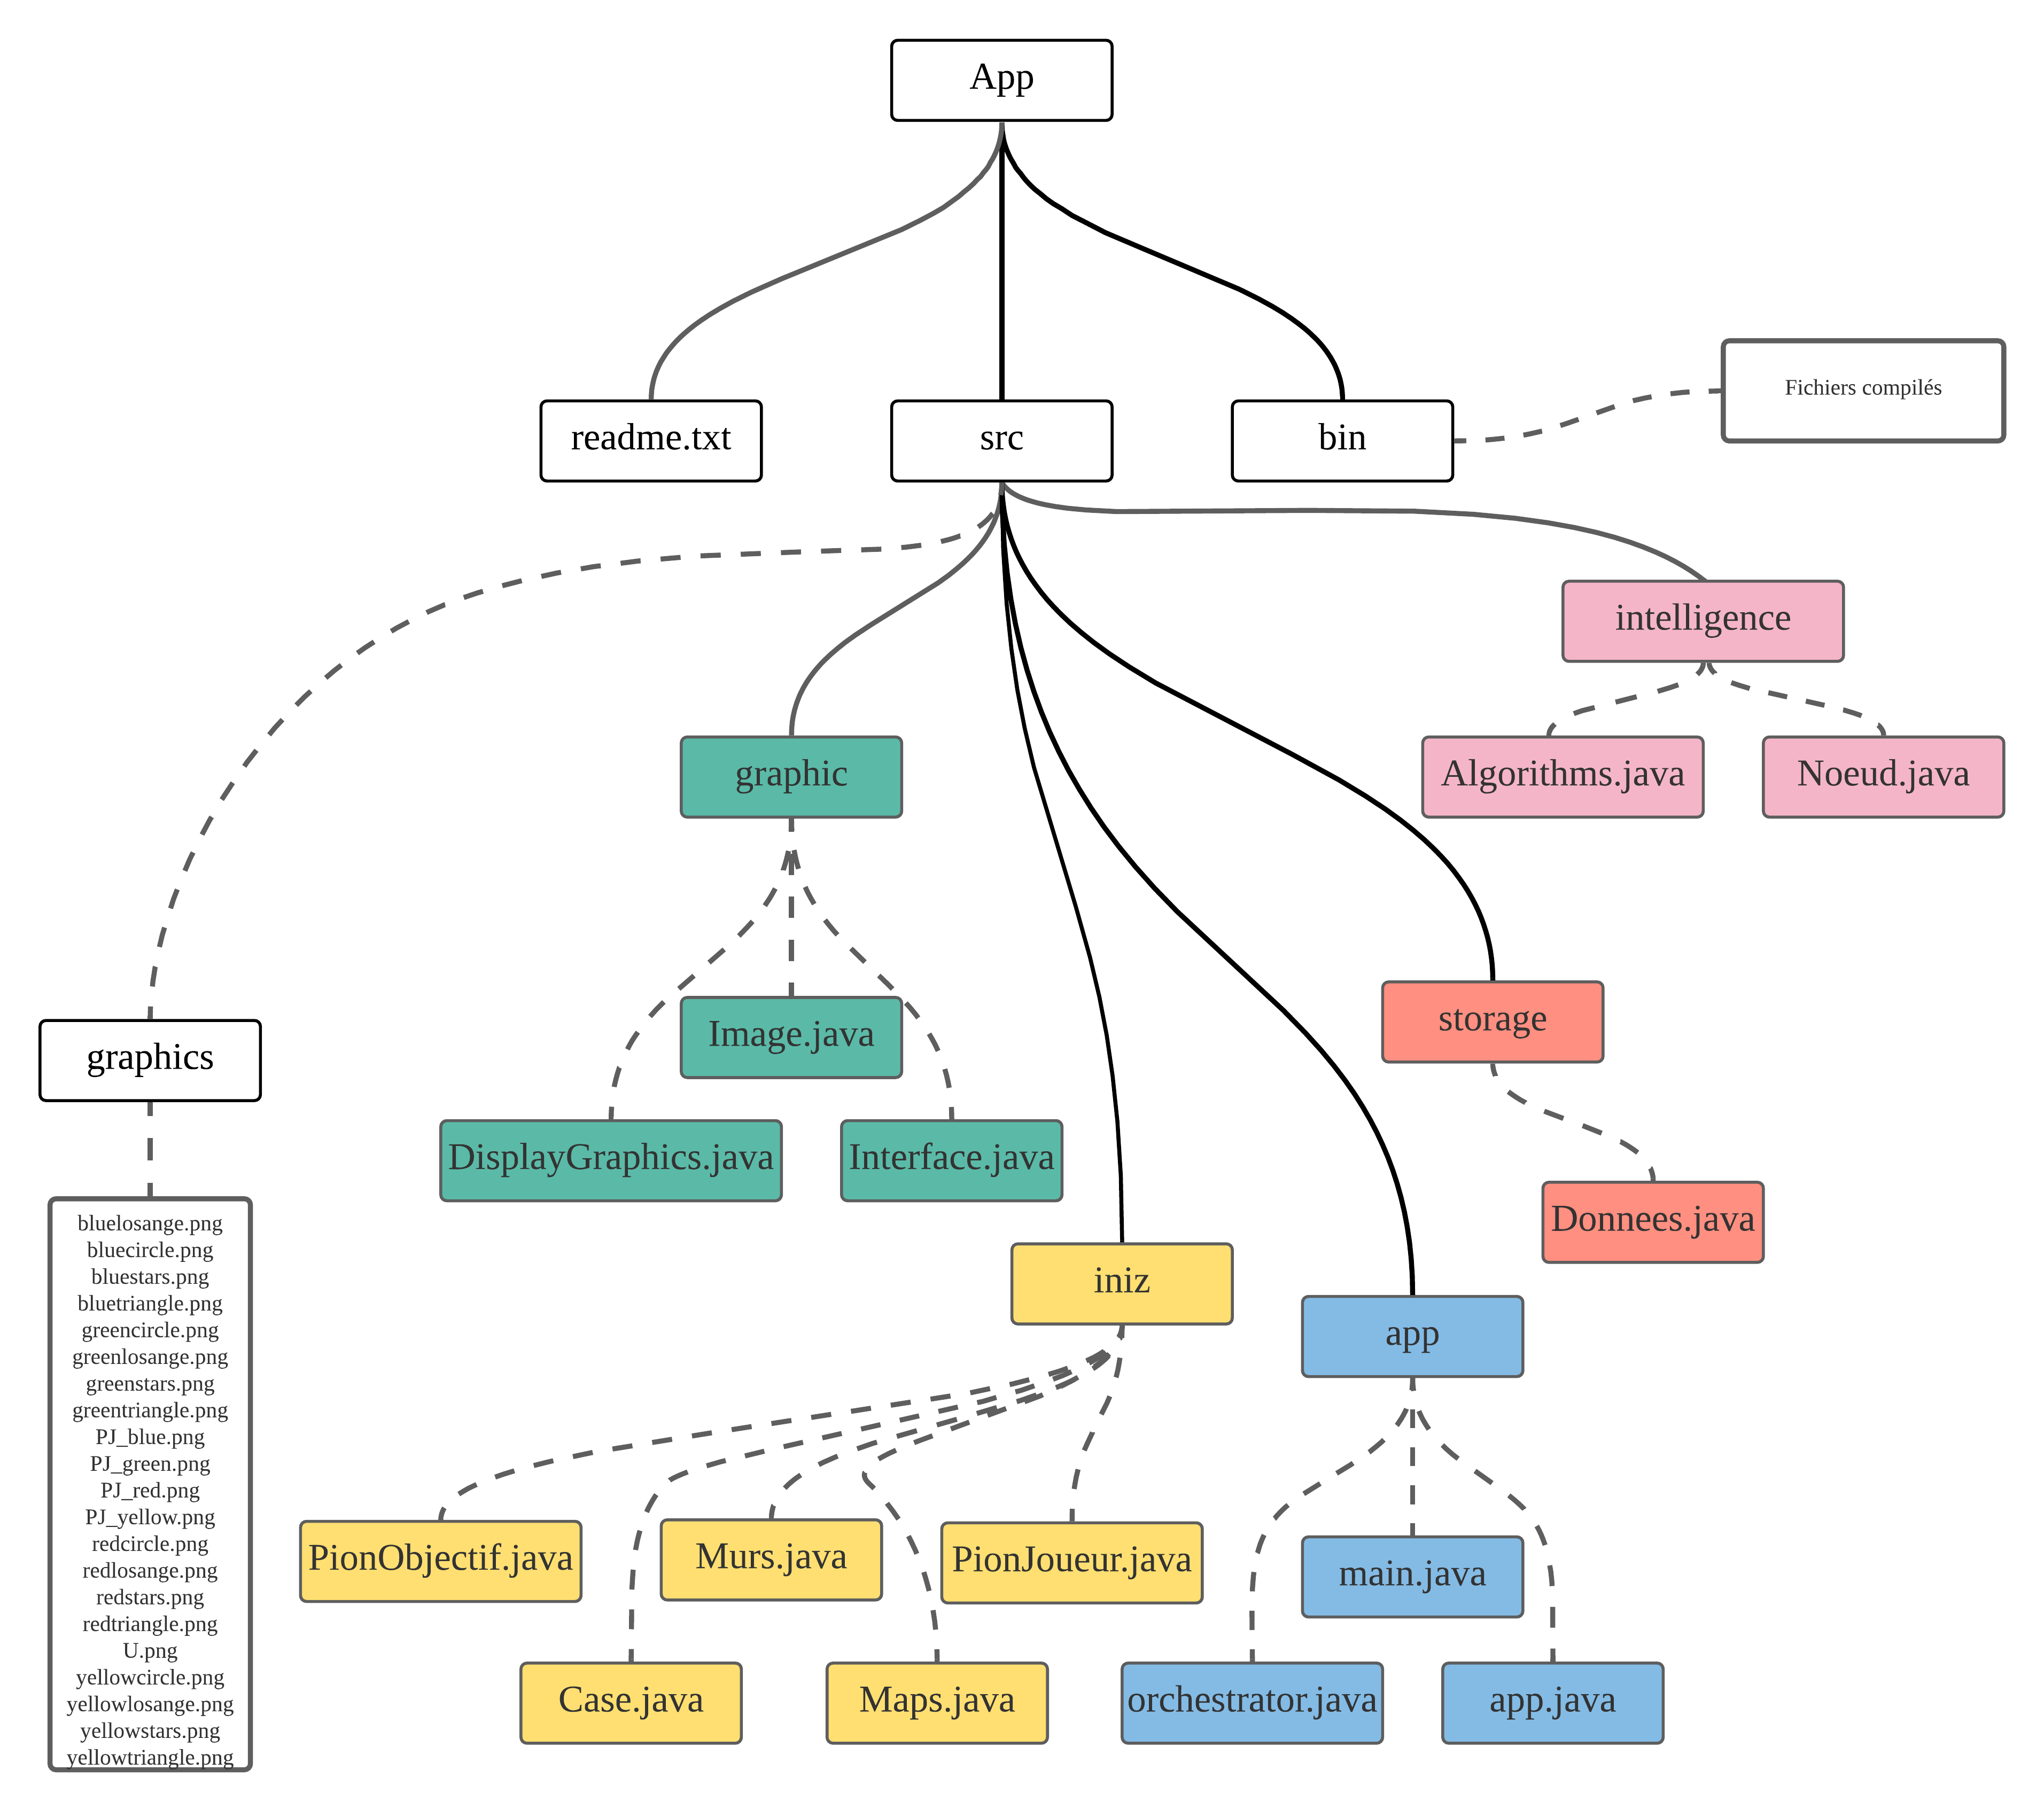
\includegraphics[width=1\textwidth]{Graphique/Arborescence.png}
    \caption{Organisation des fichiers}
    
    \label{Fig1}    
\end{figure}

\newpage

\section{Éléments techniques}

\subsection{Construction d'une carte de jeu}

La première étape lors du lancement du programme est la création d'un plateau de jeu comprenant des murs et des pions objectifs. Ce dernier est composé d'une grille de 16 par 16 cases, elle-même divisée en 4 parcelles de taille 8 par 8. Cette grille est un objet <Maps> dont la création implique un tirage aléatoire.
\newline
Dans le jeu original, chacunes des parcelles est représentées sur les faces recto/verso de quatre segment de carton, elles peuvent ainsi être assemblés coinjointement pour construire un plateau de jeu aléatoire à 64 possibilités.
\newline
\newline
Pour rester dans l'esprit de ce tirage aléatoire nous avons décidé de construire 8 parcelles statiques qui seront ensuite assemblées aléatoirement. Ces dernières sont enregistrées dans des listes de strings, chacunes de celles-ci représentant une des 8 lignes. Dans ces strings sont encodées grâces à différents caractères la nature et position des différents murs et pions objectifs.

\begin{figure}[h]
    \centering
    \ref{Fig2} 
    \includegraphics[width=0.8\textwidth]{Graphique/Création_Grille.png}
    \caption{Représentation d'une grille de jeu}
    \label{Fig2}
\end{figure}

Les bordures de nos parcelles étant ainsi enregistrées de manières statiques, elles ne peuvent être utilisées que dans leur orientation spécifiées. Nous sommes donc contraints de tirer aléatoirement pour chaque segment de plateau une des deux parcelles possibles réduisant nos possibilité à 16 grilles possibles. Nous avons cependant jugé que cette amplitude était suffisante pour conserver la rejouabilité du jeu.
\newline
\newline
Le tirage aléatoire des liste de strings, importé depuis la classe <Données> s'effectue par une méthode <aléaParcel()>, qui envoie par la suite les 4 listes de strings à la méthode <concatenate()>. Celle-ci a pour vocation de concaténer les strings de même indice, rassemblant ainsi les lignes de haut en bas. Elle retourne donc une liste de 16 strings dont chaque caractère permet d'encoder les différentes cases de la grille. Les cases sont des objets <Case> ayant comme attribut les <murs> et les <PionObjectif>
\newpage
Pour traduire cette liste de strings en un objet <Map> nous l'envoyons ensuite à la méthode éponyme <translator>. Cette dernière a pour but d'assigner à chaque caractère l'objet lui correspondant dans la grille.
\newline
 \begin{figure}[h]
    \centering
    \ref{Fig3} 
    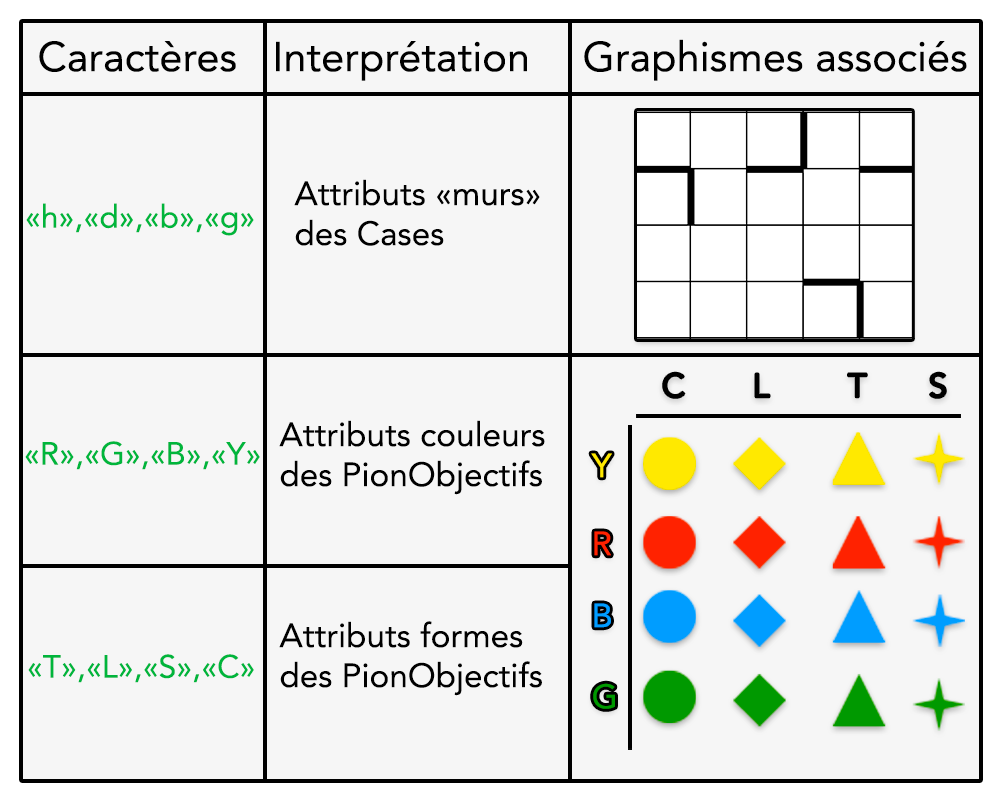
\includegraphics[width=0.55\textwidth]{Graphique/Tableau_Traduction.png}
    \caption{Tableau du convertisseur}
    \label{Fig3}
\end{figure}

La figure précédente représente la table de traduction du <translator>. À chaque partie, seulement un des 16 pions objectifs sera choisi aléatoirement pour servir de cible et sera par conséquent le seul affiché graphiquement. Ce tirage aléatoire de la cible s'effectue dans la méthode <randPO>, appelée une fois que le <translator> ait fini d'initialiser la grille du plateau de jeu.
\newline
\subsection{Placement des robots}
La dernière étape nécessaire afin d'obtenir un plateau de jeu jouable et solvable par l'algorithme est la mise en place aléatoire des <PionJoueur>, les 4 robots de couleurs distinctes.
\newline
En ce qui concerne le placement aléatoire des pions joueurs nous utilisons la méthode <aleaPJ> pour générer une position aléatoire pour l'abscisse et l'ordonnée qui devront respecter la restriction du carré central à l'aide de la méthode <alea>. Celle-ci seront contenus dans un objet <Point> de la librairie "math", cette opération sera répetée 4 fois soit le nombre de pion joueur.
\newline
Ces pions seront stockés dans un object <modele> bien que ce ne soit pas la façon de faire la plus optimisé, mais c'était necessaire pour le développement de l'IA.
\newline
\newline
Le schéma suivant représente la totalité des méthodes appelées et des objets utilisées pour la création totale d'un plateau, placement des joueurs aléatoires inclut.
\newpage

\begin{figure}[h]
    \centering
    \ref{Fig4}
    \includegraphics[width=0.95\textwidth]{Graphique/Création_Map.png}
    \caption{Création d'une carte de jeu}
    \label{Fig4}
\end{figure}

\subsection{Déplacement des robots}
Pour déplacer ces robots nous avons une méthode <movedir()> qui prend la position du robot puis renvoie la position du déplacement demandé. Avant nous avions 4 méthodes pour chaque déplacement soit <moveUp>, <moveDown>, <moveRight>, <moveLeft>, mais pour optimiser notre code nous avons pris du temps supplémentaire à essayer de la factoriser en une méthode aujourd'hui nommée <movedir()>, qui prend un point de départ, la direction 0,1,2,3 (haut,droite,bas,gauche) et une liste de points qui contient l'état des 4 pions joueurs, ajouter plus tard car nécessaire pour l'algorithme A*.
\newline
La direction nous permet de récupérer des vecteurs qui serviront à déplacer correctement le point soit en horizontal ou à la verticale et qui, a pour contrainte de se bloquer sur un mur ou un pion joueur. Pour vérifier si un pion joueur nous bloque lors du déplacement nous avons une méthode <robotCheck()> qui renvoie true s'il n'y a pas de robot à la position donnée ou alors false.
\newpage

\section{Intelligence artificielle}

\subsection{Travail de recherche}
Avant de nous lancer dans le développement ou l'ébauche de l'IA nous avons fait des recherches pour savoir comment la faire fonctionner, puis la retranscrire en code.
On a donc commencé par prendre connaissance des documents fournis avec notre sujet, pour ensuite effectuer nos propores recherches (ref:\ref{Références}).
\newline
La première chose que nous avons fait est de comprendre via wikipédia et des vidéos sur youtube ce qu'est l'heuristique pour commencer à coder les premières méthodes qui allaient calculer l'heuristique de chaque case, et ainsi obtenir une valeur estimée de la distance à parcourir entre l'objectif et le point de départ, pour comprendre le procédé voir: (ref:\ref{CD}).
\newline
Ensuite nous avons fait des recherches sur l'algorithme A* qui nous ont conduites à en faire d'autre sur ce qu'est un graph. Après avoir pris conscience de ces deux principes fondamentaux grâce à nos recherches et à l'aide de nos encadrants, nous nous sommes enfin lancés complètement dans la programmation.

\subsection{Calcul des distances}
\label{CD}

Quand on parle de calcul des distances on parle d'une estimation de coût entre un point d'arrivé et un point de départ. Dans notre cas le point d'arrivé est le pion d'objectif à atteindre alors que le point de départ est un pion de même couleur que son objectif, que le joueur peut déplacer à sa guise en respectant les contraintes. La meilleure solution est donc de calculer la distance en ayant comme point d'arrivé le pion d'objectif restant fixe jusqu'à la fin de la partie ainsi on peut obtenir un coût peu importe où notre pion joueur apparaît. 
\newline
Le nombre minimum de coups théoriques (si les pions joueurs pourraient s'arrêter sur n'importe quelle case) par rapport à l’objectif. Le point d'arrivé étant 0. Le graphisme suivant donne un exemple d’une carte de distance heuristique, appelé dans notre programme "computedMap" :

 \begin{figure}[h]
    \centering
    \ref{Fig5}
    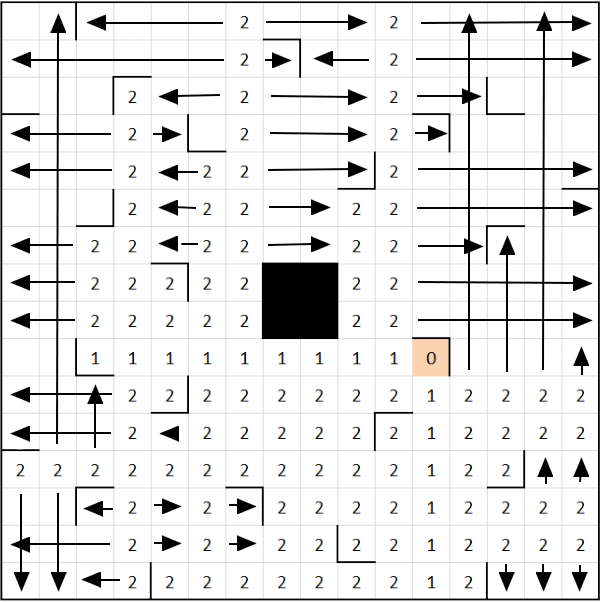
\includegraphics[width=0.45\textwidth]{Graphique/Exemple_Heuristique.png}
    \caption{Partout où il a des flèches nous insérons "3"}
    \label{Fig5}
\end{figure}

\newpage
La création de la carte heuristique se réalise à chaque lancement d'algorithme. Celle-ci est d'abord une grille remplie de '0', elle est par la suite remplie des différents coûts comme vu précedemment.
\newline
Ce remplissage s'effectue à l'aide de la méthode <delineate()> qui appelle succesivement les méthodes <depthOne> et <depthOther>. La première se charge de remplir de '1' la ligne et la colonne partant du pion d'objectif. La deuxième faisant succesivement de même pour les perpendiculaires de chaque 'profondeur', allant jusqu'à un maximum de '5' (Voir exemple de la figure précédente). 
\newline
Le schéma suivant représente la totalité des méthodes utilisées pour la création d'une carte heuristique.


\begin{figure}[h]
    \centering
    \ref{Fig6}
    \includegraphics[width=1\textwidth]{Graphique/Création_Computed.png}
    \caption{Calcul des distances}
    \label{Fig6}
\end{figure}
\newpage



\subsection{Algorithme A*}

Ayant pris connaissance des éléments ci-dessus, nous avons donc commencé par creér un constructeur "Noeud" qui contiendra les états de notre grille, avec les attributs suivant :

\begin{itemize}
    \item Une liste de points qui représente la position des quatre pions joueurs, ordonnée par les couleurs respectives : rouge, bleu, vert, jaune pour les index 0,1,2,3.
    \item Un point nommé "target" qui est le pion joueur qui doit atteindre la cible.
    \item \label{calcule} Le coût "cost" qui sera une addition de la profondeur et de sa distance heuristique stocker dans la computedMap
    \item La profondeur "count" qui sera la profondeur de notre Noeud, autrement dit le nombre de coûts qui ont été fait depuis l'état initial.
    \item Un Noeud "parent" qui nous permettra de récuperer le Noeud précédent, ce parent peut donc s'appeler aussi "previous".
\end{itemize}

En ayant tous ces éléments à notre disposition nous pouvons commencer à créer le premier Noeud qui contiendra l'état initial à partir duquel tous les autres Noeuds seront créés grâce à la méthode "makeChildren", qui en plus de les créer les ajoutera dans l'openList, une liste contenant tous les Noeuds que nous allons créer. Par exemple voici ce que donnerait au premier appel cette méthode dans la mesure ou tous les pions des joueurs peuvent se déplacer dans les 4 directions sans limite : 

 \begin{figure}[h]
    \centering
    \ref{Fig7}
    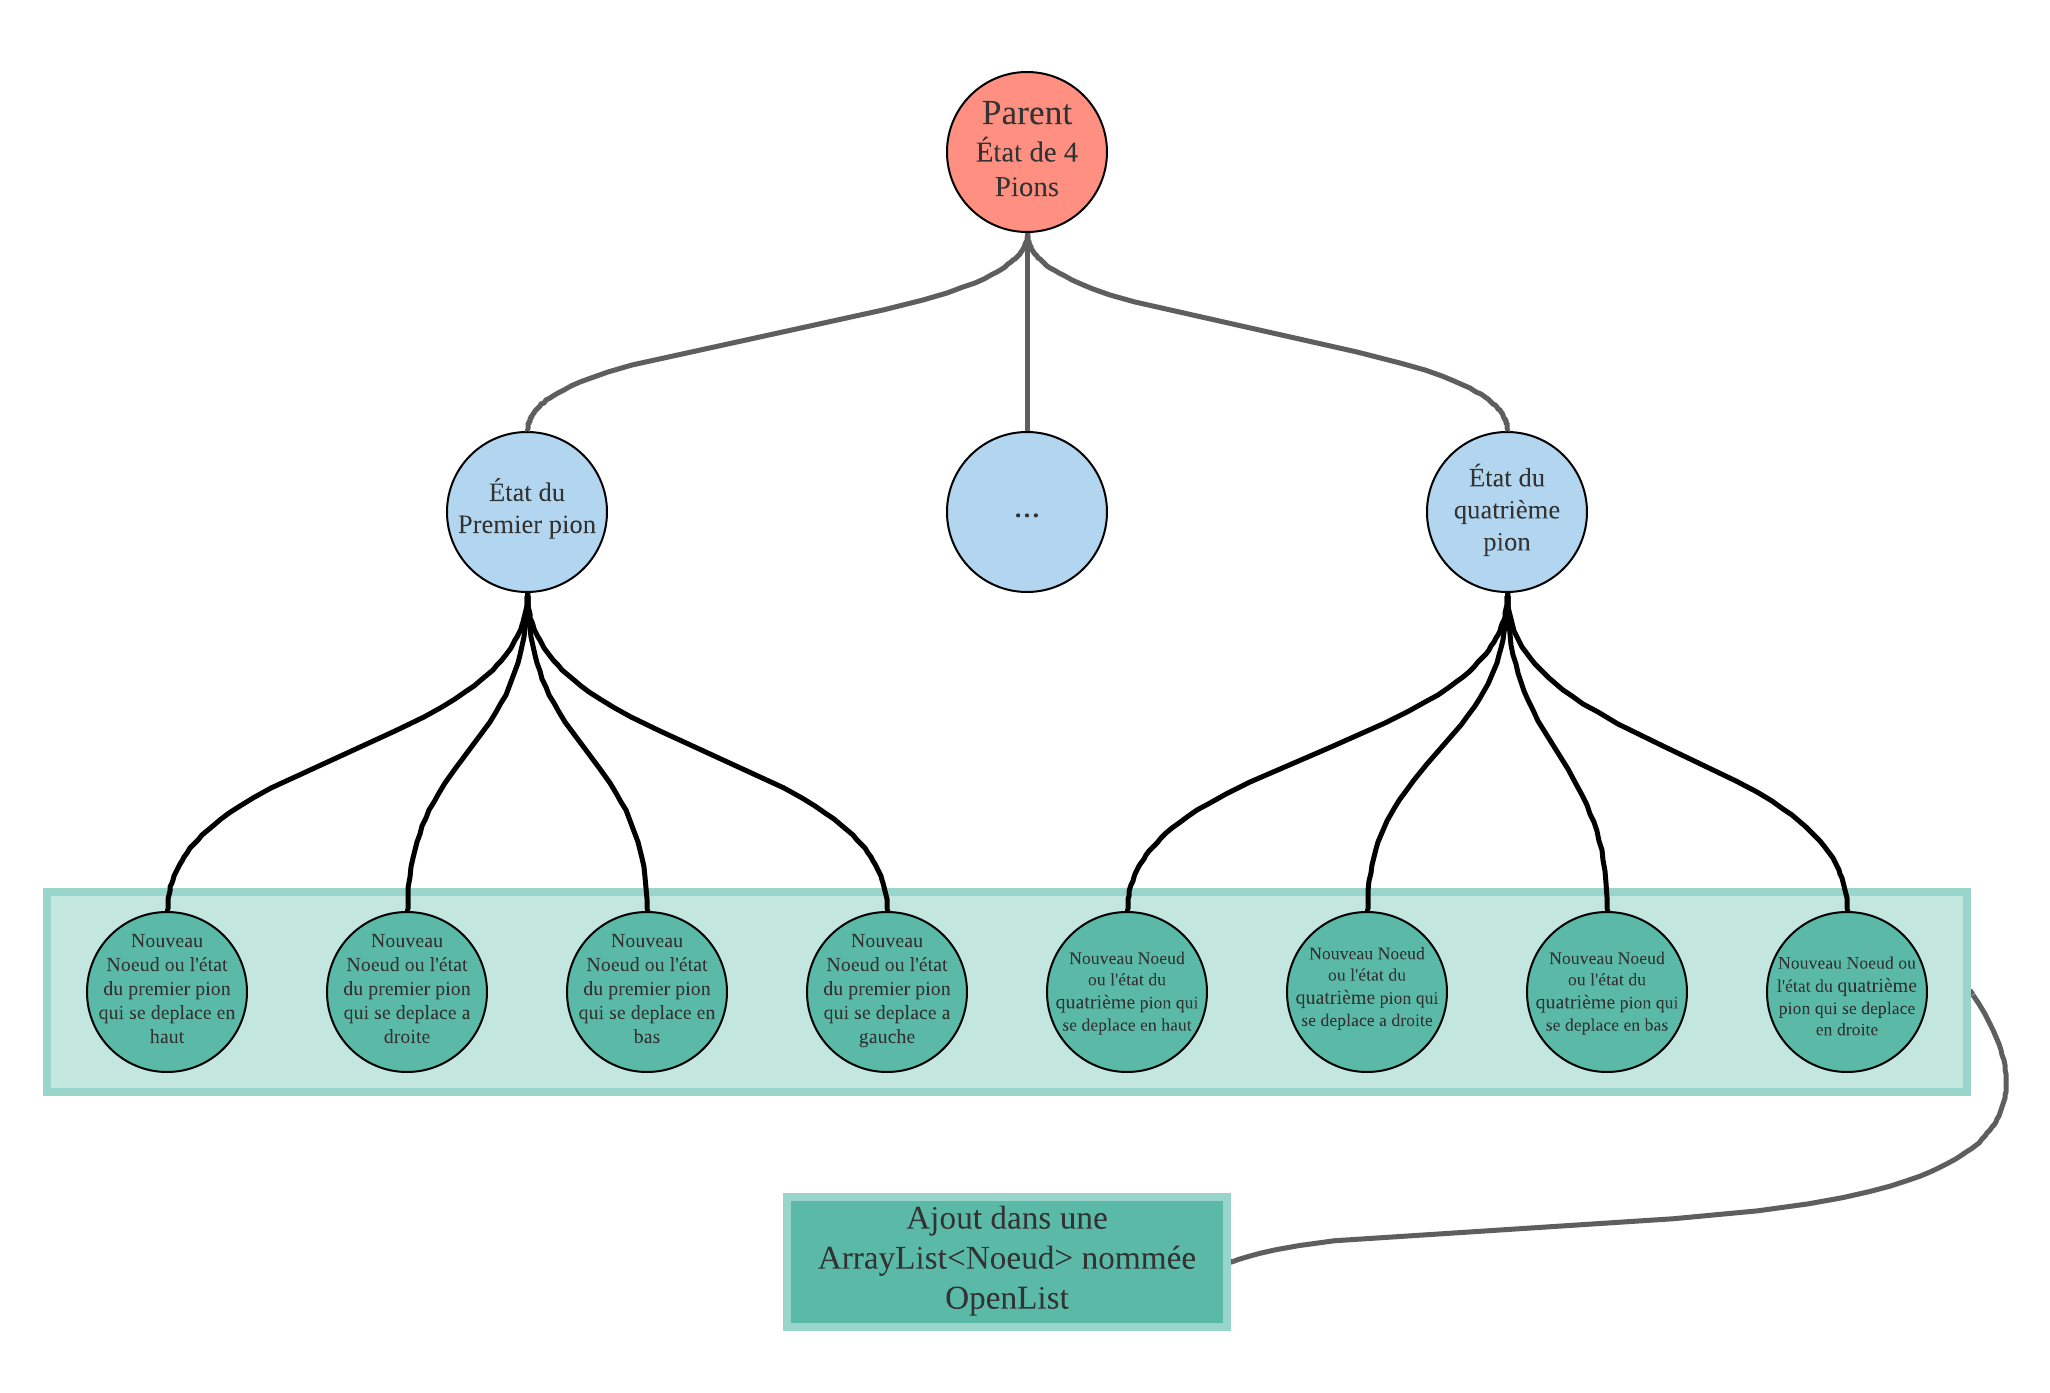
\includegraphics[width=1\textwidth]{Graphique/MakeChildrens.png}
    \caption{Récupération de nouveaux états a partir d'un Noeud}
    \label{Fig7}
\end{figure}

\newpage

Dans un second temps, nous allons modifier chaque noeud ne contenant pas de coût, en suivant le calcul \ref{calcule} expliqué plus haut. Ensuite nous aurons un noeud tampon qui nous servira à sélectionner le noeud ayant le plus petit coût et un état dans lequel le pion joueur devant atteindre l'objectif se déplace, parmi notre liste "openList" . 
\newline
Une fois ceci achevé nous rentrerons dans une boucle (while) qui aura pour condition une méthode <checkOver()> qui renverra un boolean pour stopper la boucle. Le noeud tampon nommé "selected", est l'état avec le coût le plus bas pour atteindre le pion d'objectif.
\newline
La méthode <checkOver> supprimera  également  le Noeud tampon de l'openList, et l'ajoutera dans la "closedList", une liste renfermant les noeuds déjà explorés ou inutiles.  La boucle sortira donc uniquement dès qu'un chemin sera trouvé, chemin que l'on récupérera grâce à une méthode qui s'appelle <getPath()>.
\newline
Celle-ci récupérera tous les parents liés au noeud final, et chacun d'entres eux sera ajouté dans une liste de noeud nommé "path". La solution sera ensuite inversée en utilisant une méthode de la librairie "Collection"  et ainsi récuperer tous les états nécessaire à reproduire pour gagner. Ci-dessous un schéma illustratif: 

 \begin{figure}[h]
    \centering
    \ref{Fig8}
    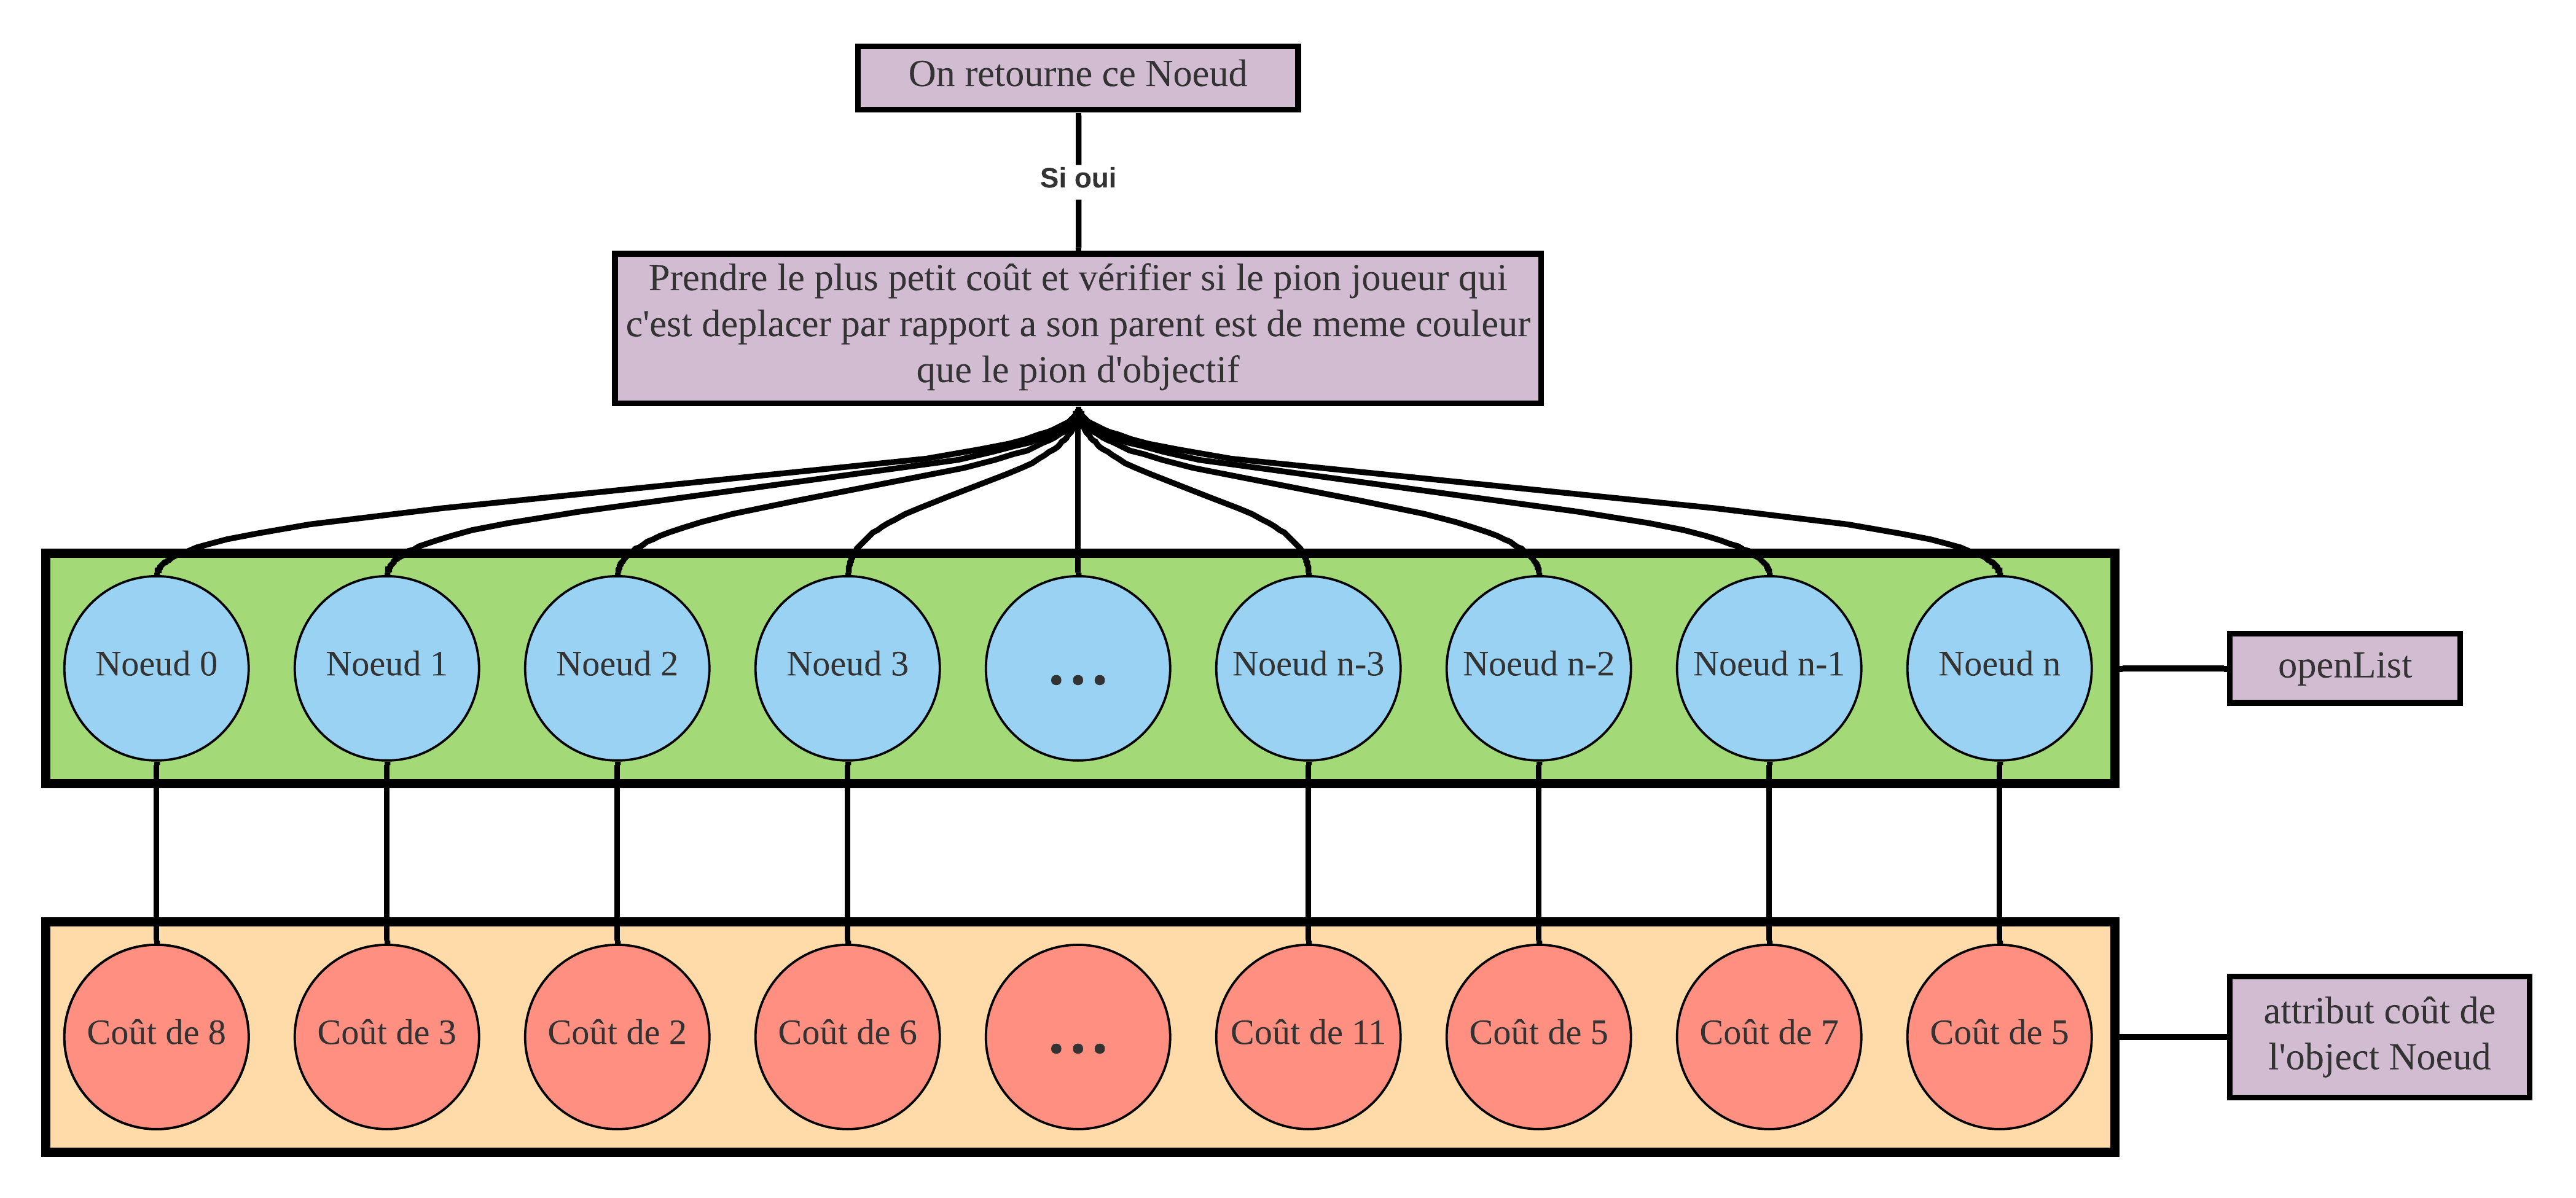
\includegraphics[width=1\textwidth]{Graphique/Noeud.png}
    \caption{Récupération de nouveaux états à partir d'un Noeud}
    \label{Fig8}
\end{figure}

\newpage
\section{Conclusion}

\subsection{Objectifs remplis}

Au cours de la réalisation de ce projet nous avons été bloqués par plusieurs problèmes que nous avons rencontrés. Nous voulions le moins possible avoir des méthodes rededondantes, ainsi nous avons passés une grande partie du temps à trouver des solutions pour les concaténer, pour qu'une fois avancé dans le code, nous puisions les ajuster plus facilement afin de faire des manipulations sans changer la majorité du code.
\newline
Mise à part les longues heures à isoler et résoudre des problèmes en l'occurence sur la méthode de déplacement ou encore l'implémentation de l'algorithme A*, nous pensons avoir fait de notre mieux avec le temps imparti, les contraintes que nous avions et la documentation que nous avons trouvée sur le sujet. Donc nous pouvons dire que oui, nous avons en grande partie remplis les objectifs malgrès la contrainte du temps sans quoi nous aurions pu ajouter des améliorations que nous allons voir sur le point suivant.

\subsection{Améliorations possibles}

En ce qui concerne les améliorations, nous avons une grande quantité d'idées pour l'affichage, ou encore l'algorithme. Nous allons donc énumérer ici les améliorations auxquelles nous avons pensé :


\begin{itemize}
    \item Lorsque l'on place la souris sur un pion joueur on a la possibilité de voir en surbrillance les directions vers lesquelles on peut se déplacer.
    \item Quand on veut trouver la solution en appuyant sur le bouton résoudre, on pourrait faire apparaître un chemin en surbrillance. Cela permettrait aussi de ne plus utiliser le terminal de commandes.
    \item Ajouter une gestion des erreurs, nous y avons pensé mais n'avons pas pris la décision de prendre du temps supplémentaire pour l'implémenter, autrement cette amélioration permettrait d'identifier les problèmes plus rapidement. 
    \item Et enfin évidemment, ajouter à notre algorithme A* la possibilité de trouver les solutions où l'on doit obligatoirement se servir de 2 pions joueurs. L'ajout de cette amélioration augmenterait aussi considérablement le nombre de calculs executés pour trouver la solution d'un point A à un point B.
\end{itemize}


\subsection{Remerciement spécial}

Nous souhaitons remercier particulièrement notre encadrant de projet, Pr.Yann Mathet qui a su malgré les circonstances des cours prendre le temps de bien répondre pédagogiquement à nos questions ce qui nous a permis d'avoir une rythme de travail très linéaire, ainsi qu'à notre enseignant en Complément POO Mr.JACQUIER Yohann qui a pris le temps hors-cours de nous aiguiller sur certains problèmes que nous avons rencontrés.

\newpage
\section{Références}
\label{Références}


\begin{enumerate}
    \item Distance de Manhattan : \url{https://fr.wikipedia.org/wiki/Distance_de_Manhattan}
    \item Wikipédia Algorithms A* : \url{https://en.wikipedia.org/wiki/A*_search_algorithm}
    \item Youtube Pathfinding : \url{https://www.youtube.com/watch?v=-L-WgKMFuhE&t}
    \item Solving Ricochet Robots Conférence : \url{https://www.youtube.com/watch?v=fvuK0Us4xC4}
    \item Règle du jeu :
    \url{http://maludo.chez.com/regles/RASEN.pdf}
    \item Image d'un plateau de jeu Ricochet Robot \url{http://www.jeuxadeux.com/images/ricochet_robots_2_gd.jpg}
    \item Diaporama pour faire un solver de Ricochet Robot \url{https://speakerdeck.com/fogleman/ricochet-robots-solver-algorithms}
    \item Ricochet Robot en ligne
    \url{http://www.ricochetrobots.com/RR.html}
    
\end{enumerate}
\end{document}
